% ======================= Pre-Amble =========================
      
%Format
\documentclass[11pt, oneside]{article}   	% use "amsart" instead of "article" for AMSLaTeX format 
                     						%imports package {article} and specify option(s) [11pt, oneside]
\usepackage{geometry}                		% See geometry.pdf to learn the layout options. There are lots. 
    \geometry{letterpaper}                   		% ... or a4paper or a5paper or ... 
    %\geometry{landscape}                		% Activate for rotated page geometry

\usepackage[parfill]{parskip}    		        % Activate to begin paragraphs with an empty line rather than an indent

    %Colours
    \usepackage{graphicx, subcaption}
    \usepackage[usenames, dvipsnames]{color}     % font colour:    \textcolor{<colour>}{text}
          									%highlight text:  \colorbox{<color>}{text}
    \usepackage{soul}						%highlight text: \hl{}     %only  yellow								
    									%list of colours: https://www.sharelatex.com/learn/Using_colours_in_LaTeX
    									
    %Bullets
    \usepackage{enumerate}     %specify type of enumeration: \being{enumerate}[<type of enumeration>]
    
    %Footnote Spacing
    \setlength{\footnotesep}{0.4cm}                  %specify spacing b/w footnotes
    \setlength{\skip\footins}{0.6cm}                    % space b/w footnotes and textbody


%Mattematics
    %American Mathematics Society packages
    \usepackage{amsmath}	   %math
    \usepackage{amssymb}       %symbols
    \usepackage{amsthm}          %theorems

    %QED
    \newcommand*{\QEDA}{\hfill\ensuremath{\blacksquare}}         %make qed filled square:    \QEDA
    \newcommand*{\QEDB}{\hfill\ensuremath{\square}}               %make qed empty square: \QEDB 
    
    \renewcommand\qedsymbol{\ensuremath{\blacksquare}}		%Proof environment


%Figures
\usepackage{caption}
\captionsetup[figure]{labelfont=bf}    %make figure labels boldface
\captionsetup[table]{labelfont=bf}     %make table labels boldface

\usepackage[hidelinks]{hyperref}                % Allows for clickable references

    %Tables
    \usepackage[none]{hyphenat}                    % Stops breaking-up words in a table (i.e. no hyphens)                                                             
    
    \usepackage{array}   
        \newcolumntype{x}[1]{>{\centering\let\newline\\\arraybackslash\hspace{0pt}}p{#1}}       %center fixed column width: x{<len>}                      
        \newcolumntype{$}{>{\global\let\currentrowstyle\relax}}                                                   % let us apply things (e.g. bold/italicize) to entire row            
        \newcolumntype{^}{>{\currentrowstyle}}
        \newcommand{\rowstyle}[1]{\gdef\currentrowstyle{#1} #1\ignorespaces}
    
    %Images
    \graphicspath{ {images/} }                          %directory that your images are located in within your current directory
    
    %Diagrams
    \usepackage[latin1]{inputenc}
    \usepackage{tikz}
    	\tikzset{line/.style={-latex'}}
        \usepackage{tkz-berge}
        \usetikzlibrary{shapes,arrows}
        \usetikzlibrary{patterns}			%Specify colours of stuff (e.g. vertices): 
        								%	-> set style: \tikzset{VertexStyle/.append style = {minimum size = 8pt, inner sep = 0pt}} 
								%	-> change individual vertices: \AddVertexColor{white}{1,2} 


%Bibliography
\usepackage[numbers,sort&compress]{natbib}   %for multiple references: sorts  (i.e. [1,2] NOT [2, 1] )
                                           				  %                                     compresses (i.e. [1-3] )
\usepackage[nottoc]{tocbibind}                            %add bibliography to table of contents


%Miscellaneous
\usepackage{dirtytalk}    %quotations: use \say  


%================== Header & Footer =========================
\usepackage{fancyhdr}
\usepackage{lastpage}      %ensures you can reference LastPage (i.e. Page 2 of 10)

\renewcommand{\headrulewidth}{0.4pt}		%Decorative Header line: thickness={0.4pt}
\renewcommand{\footrulewidth}{0.4pt}		%Decorative Footer line: thickness={0.4pt}

\setlength{\headheight}{13.6pt} 		%space b/w top of page & header
\setlength{\headsep}{0.3in}		%space b/w page header and body

%Make Header & Footer    
\pagestyle{fancy}
    \lhead{Stephanie Knill} 		% controls the left corner of the header
    \chead{} 					% controls the center of the header
    \rhead{} 					% controls the right corner of the header
    \lfoot{} 					% controls the left corner of the footer
    \cfoot{Page~\thepage\ of \pageref{LastPage}} 				% controls the center of the footer
    												%Page~\thepage\  if just want Page x
    \rfoot{}			 		% controls the right corner of the footer

% =============================== Document ===================================
\begin{document}

% Title Page
\title{MATH 442 --- Assignment 11 \\
\line(1,0){360} \\              %(slope x, y){length of line}
}
\author{
Stephanie Knill \\
54882113 \\
Due: March 31, 2016}

\date{}                   % Activate:  display a given date (e.g. {August 4} ) or no date (empty {} )
                                    %No activate: display current date
\maketitle

%\thispagestyle{empty}                   %Remove header from this (first) page. Change empty -> plain to keep numbering
%								-> Doesn't matter in this case (b/c title page)
%\cleardoublepage


% ================= Questions ================

\section*{Question 61}

Let $n \geq 3$
\begin{enumerate}[\quad(a)]
	\item \emph{Show the number of pairs $(T,e)$ where $T$ is a spanning tree of $K_n$ and $e$ is an edge of $T$ is $n^{n-2}(n-1)$.}
	
	By our in-class Corollary 6, we know that the number of spanning trees in $K_n$ is $T=n^{n-2}$. By Homework 9, we know that the number of edges $e$ in a tree of $n$ vertices is given by $e=n-1$. Multiplying these together gives us $n^{n-2}(n-1)$, the number of pairs $(T,e)$.
	
	\item \emph{Show that the number of spanning trees of $K_n$ containing a specific edge is $2n^{n-2}$.}
	
	To find the number of spanning trees of $K_n$ containing a specific edge, we must take the number of pairs $(T,e)$ and multiply this by the probability of selecting any edge in $K_n$. Since there are $\frac{n(n-1)}{2}$ edges in  $K_n$, the probability of selecting any edge is $\frac{2}{n(n-1)}$. Multiplying this by the result found in part a) gives us
	$$n^{n-2}(n-1) \cdot \frac{2}{n(n-1)} = \frac{2 n^{n-2}}{n} = 2n^{n-3}$$
	
	\item \emph{Show that for some edge $e$ in $K_n$, we have $\tau(K_n-e) = (n-2)n^{n-3}$}
	
	Deleting any edge $e$ from $K_n$ and calculating the number of spanning trees of the resulting graph $K_n-e$  is equivalent to calculating all possible spanning trees of $K_n$ and subtracting the number of spanning trees that contain edge $e$. Thus we have
	\begin{align*}
		\tau(K_n - e) & = \tau(K_n) - 2n^{n-3} \\
		& = n^{n-2} - 2n^{n-3} \\
		& = (n-2)n^{n-3}
	\end{align*}
\end{enumerate}

\section*{Question 62}

For the following graphs Figure \ref{q2}, we may start at the vertex labelled 1 and conduct a Depth First Search (blue) and a Breadth First Search (red)
\begin{figure}[h]           
            \centering
            \begin{subfigure}[b]{0.45\columnwidth}
            	\centering
             	 \begin{tikzpicture}[scale=0.75,transform shape]
        		
        		\GraphInit[vstyle=Classic]					%Make vertice labels outside it
        		%\SetVertexNoLabel							%No vertice labels
        		\tikzset{VertexStyle/.append style = {fill=black, circle}}		%Set vertex style        		
			\Vertex [x=0,y=0]{1}
			\SetVertexNoLabel	
			\Vertex [x=1.5,y=0,]{2}
			\Vertex [x=3,y=1]{3}
			\Vertex [x=3,y=-1,]{4}
			\Vertex [x=4.5,y=0,]{5}
			\Vertex [x=6, y=0,]{6}
			\Vertex [x=6,y=1,]{7}
			\Vertex [x=6,y=-1,]{8}
			\Vertex [x=7.5,y=0,]{9}
			
        		%\AddVertexColor{white}{1,2} 					%Change individual vertex type         
        			\path [thick] (1) edge (2);			%arrows: [line];     label: {$label}$
			\path [thick] (2) edge (3);
			\path [thick] (2) edge (4);
			\path [thick] (3) edge (5);
			\path [thick] (4) edge (5);
			\path [thick] (6) edge (5);
			\path [thick] (7) edge (5);
			\path [thick] (8) edge (5);
			\path [thick] (7) edge (9);
			\path [thick] (6) edge (9);
			\path [thick] (8) edge (9);
			
            	\end{tikzpicture}
		\label{Graph1}
            \end{subfigure}
           \begin{subfigure}[b]{0.45\columnwidth}
            	\centering
             	 \begin{tikzpicture}[scale=0.75,transform shape]
        		
        		\GraphInit[vstyle=Classic]					%Make vertice labels outside it
        		%\SetVertexNoLabel							%No vertice labels
        		\tikzset{VertexStyle/.append style = {fill=black, circle}}		%Set vertex style        		
			\Vertex [x=5.5,y=0]{1}
			\SetVertexNoLabel	
			\Vertex [x=0,y=0,]{2}
			\Vertex [x=1,y=1,]{3}
			\Vertex [x=2,y=0,]{4}
			\Vertex [x=2,y=2,]{5}
			\Vertex [x=3.5, y=0,]{6}
			\Vertex [x=3.5,y=2,]{7}
			\Vertex [x=4.5,y=1]{8}
        		%\AddVertexColor{white}{1,2} 					%Change individual vertex type
            
        			\path [thick] (1) edge (8);			%arrows: [line];     label: {$label}$
			\path [thick] (2) edge (3);
			\path [thick] (5) edge (3);
			\path [thick] (4) edge (3);
			\path [thick] (6) edge (3);
			\path [thick] (5) edge (7);
			\path [thick] (4) edge (6);
			\path [thick] (6) edge (8);
			\path [thick] (7) edge (8);
			\path [thick] (4) edge (8);
            	\end{tikzpicture}
		\label{Graph2}
            \end{subfigure}
           
            \caption{Depth First Search and Breadth First Search of various graphs.}
            \label{q2}
        \end{figure}

\section*{Question 63}

For the weighted graph $G$ (Figure \ref{q63}), we can compute the shortest distance from vertex $A$ to each vertex (Table \ref{paths}).
	\begin{figure}[h]
	\centering
        \begin{tikzpicture}[scale=0.75,transform shape]		
		%\GraphInit[vstyle=Classic]					%Make vertice labels outside it
		%\SetVertexNoLabel							%No vertice labels
		\tikzset{VertexStyle/.append style = {circle}}		%Set vertex style
			%\AddVertexColor{white}{1,2} 					%Change individual vertex type
			\Vertex [x=0,y=0,]{A}	
			\Vertex [x=3,y=3,]{B}
			\Vertex [x=3,y=0]{C}
			\Vertex [x=3,y=-3]{D}
			\Vertex [x=8,y=3]{E}
			\Vertex [x=8, y=0,]{F}
			\Vertex [x=8,y=-3]{G}
			\Vertex [x=11,y=0]{H}
    		
		\path [solid] (A) edge node[midway,above] {2} (B);					%arrows: [line];     label: {$label}$
		\path [solid] (A) edge node[midway,above] {4} (C);
		\path [solid] (A) edge node[midway,below] {6} (D);
		\path [solid] (B) edge node[midway,above] {8} (E);
		\path [solid] (B) edge node[midway,above] {3} (F);
		\path [solid] (B) edge node[midway,left] {3} (C);
		\path [solid] (C) edge node[midway,above] {10} (F);
		\path [solid] (C) edge node[midway,above] {1} (G);
		\path [solid] (C) edge node[midway,left] {2} (D);
		\path [solid] (D) edge node[midway,below] {2} (G);
		\path [solid] (E) edge node[midway,right] {1} (F);
		\path [solid] (E) edge node[midway,above] {9} (H);
		\path [solid] (F) edge node[midway,above] {3} (H);
		\path [solid] (F) edge node[midway,right] {4} (G);
		\path [solid] (G) edge node[midway,below] {5} (H);
		
    	\end{tikzpicture}  
        \caption{Shortest paths in a weighted graph $G$.}
        \label{q63}
	\end{figure}
	
 	\begin{table}[h]                                          %optional argument: place figure/table here (h), top (t), page of floats (p)
        \begin{center}
        \begin{tabular}{c | ^c|^c}  
            %\multicolumn{3}{c}{\textbf{Shortest Paths in $G$}} \\
            %[0.5cm]              %row skip \\[<len>], where <len> is any length
            \rowstyle{\bfseries} Start \& End & Distance & Path  \\          
            \hline  				
            $A \to A$ & 0 & \\
            $A \to B$ & 2 & $AB$\\
            $A \to C$ & 4 & $AC$\\
            $A \to D$ & 6 & $AD$ or $ACD$\\
            $A \to E$ & 6 & $ABFE$\\
            $A \to F$ & 5 & $ABF$\\
            $A \to G$ & 5 & $ACG$ \\	
            $A \to H$ & 8 & $ABFH$\\	
        \end{tabular}
        \end{center}
        \caption{Table of shortest path distance between vertex $A$ and the remaining vertices in graph $G$.}
        \label{paths}
        \end{table}



\section*{Question 64}

Assign integer weights to the edges of $K_n$. Prove that the total weight on every cycle is even if and only if the total weight on every triangle (i.e. cycle of length 3) is even.
\begin{proof}
$\Rightarrow$ Assume that the total weight of every cycle is even. Since a triangle is a cycle of length 3, then the total weight is also even.

$\Leftarrow$ Assume that the total weight on every triangle is even. We will do an induction over the size $m$ of a cycle.

\textbf{Base Case:} For a cycle of size $m =3$, we have a triangle. By our initial assumption, our cycle has an even total weight.

\textbf{Induction Step:} Assume that the statement holds true for cycles of size $3 < m < k$. For a cycle $C$ of size $m=k$, let us choose any path of length 3 from vertices $u$ to $v$, traversing edges $a$ and $b$. Deleting edges $a$ and $b$ from our cycle and joining vertices $u$ and $v$ by a new edge $c$, we have by our induction assumption a cycle $D$ of even weight. Since we also have a triangle of edges $a, b$, and $c$ we know that this cycle is also of even weight. Thus the parity of the weights $W(a) + W(b)$ and $W(c)$ must be the same. Therefore the cycles $D$ and $C$ also have weights of the same parity, so $C$ is of even weight.

\textbf{Conclusion:} By the principle of induction,  the statement is true for all $n \geq 3$.

\end{proof}

\cleardoublepage
\section*{Question 65}

Find a simple connected graph and assign the edge weights (1,1,1,2,2,3,3,3) in two ways: one way so the minimal spanning tree is unique and another way so it is not unique

\emph{Minimal Spanning Tree Unique}

Here our simple connected graph $G$ is depicted in Figure \ref{q65 G} and its unique minimal spanning tree in Figure \ref{q65 Gspan}.
\begin{figure}[h]           
            \centering
             \begin{subfigure}[b]{0.45\columnwidth}
            	\centering
             	 \begin{tikzpicture}[scale=0.75,transform shape]
        		
        		\GraphInit[vstyle=Classic]					%Make vertice labels outside it
        		\SetVertexNoLabel							%No vertice labels
        		\tikzset{VertexStyle/.append style = {fill=black, circle}}		%Set vertex style        		
			\Vertex [x=0,y=0]{1}
			\Vertex [x=2,y=0,]{2}
			\Vertex [x=1,y=2,]{3}
			\Vertex [x=-.5,y=2,]{4}
			\Vertex [x=2.5,y=2,]{5}
			\Vertex [x=1, y=4]{6}
			\Vertex [x=0,y=3.5,]{7}
			\Vertex [x=2,y=3.5]{8}
        		%\AddVertexColor{white}{1,2} 					%Change individual vertex type
            
        			\path [thick] (1) edge node[midway,below] {1} (2);			%arrows: [line];     label: {$label}$
			\path [thick] (2) edge node[midway,right] {3} (3);
			\path [thick] (1) edge node[midway,left] {1} (3);
			\path [thick] (3) edge node[midway,below] {3} (4);
			\path [thick] (3) edge node[midway,below] {3} (5);
			\path [thick] (3) edge node[midway,right] {1} (6);
			\path [thick] (3) edge node[midway,left] {2} (7);
			\path [thick] (3) edge node[midway,right] {2} (8);
            	\end{tikzpicture}
            \caption{Graph $G$}
            \label{q65 G}
        \end{subfigure}
         \begin{subfigure}[b]{0.45\columnwidth}
            	\centering
             	 \begin{tikzpicture}[scale=0.75,transform shape]
        		\GraphInit[vstyle=Classic]					%Make vertice labels outside it
        		\SetVertexNoLabel							%No vertice labels
        		\tikzset{VertexStyle/.append style = {fill=black, circle}}		%Set vertex style        		
			\Vertex [x=0,y=0]{1}
			\Vertex [x=2,y=0,]{2}
			\Vertex [x=1,y=2,]{3}
			\Vertex [x=-.5,y=2,]{4}
			\Vertex [x=2.5,y=2,]{5}
			\Vertex [x=1, y=4]{6}
			\Vertex [x=0,y=3.5,]{7}
			\Vertex [x=2,y=3.5]{8}
        		%\AddVertexColor{white}{1,2} 					%Change individual vertex type
            
        			\path [thick] (1) edge node[midway,below] {1} (2);			%arrows: [line];     label: {$label}$
			%\path [thick] (2) edge node[midway,right] {3} (3);
			\path [thick] (1) edge node[midway,left] {1} (3);
			\path [thick] (3) edge node[midway,below] {3} (4);
			\path [thick] (3) edge node[midway,below] {3} (5);
			\path [thick] (3) edge node[midway,right] {1} (6);
			\path [thick] (3) edge node[midway,left] {2} (7);
			\path [thick] (3) edge node[midway,right] {2} (8);
            	\end{tikzpicture}
            \caption{Unique minimal spanning tree of $G$.}
            \label{q65 Gspan}
            \end{subfigure}
        \end{figure}

\emph{Minimal Spanning Tree Not Unique}

Here our simple connected graph $H$ is depicted in Figure \ref{q65 H} and its non-unique minimal spanning trees in Figure \ref{q65 Hspan}.

\begin{figure}[h]           
            	\centering
             	 \begin{tikzpicture}[scale=0.75,transform shape]
        		
        		\GraphInit[vstyle=Classic]					%Make vertice labels outside it
        		\SetVertexNoLabel							%No vertice labels
        		\tikzset{VertexStyle/.append style = {fill=black, circle}}		%Set vertex style        		
			\Vertex [x=0,y=0]{1}
			\Vertex [x=2,y=0,]{2}
			\Vertex [x=1,y=2,]{3}
			\Vertex [x=-.5,y=2,]{4}
			\Vertex [x=2.5,y=2,]{5}
			\Vertex [x=1, y=4]{6}
			\Vertex [x=0,y=3.5,]{7}
			\Vertex [x=2,y=3.5]{8}
        		%\AddVertexColor{white}{1,2} 					%Change individual vertex type
            
        			\path [thick] (1) edge node[midway,below] {3} (2);			%arrows: [line];     label: {$label}$
			\path [thick] (2) edge node[midway,right] {3} (3);
			\path [thick] (1) edge node[midway,left] {3} (3);
			\path [thick] (3) edge node[midway,below] {1} (4);
			\path [thick] (3) edge node[midway,below] {1} (5);
			\path [thick] (3) edge node[midway,right] {1} (6);
			\path [thick] (3) edge node[midway,left] {2} (7);
			\path [thick] (3) edge node[midway,right] {2} (8);
            	\end{tikzpicture}
            \caption{Graph $H$}
            \label{q65 H}
        \end{figure}
        
        
        
\begin{figure}[h]     
         \begin{subfigure}[b]{0.3\columnwidth}
            	\centering
             	 \begin{tikzpicture}[scale=0.75,transform shape]
        		\GraphInit[vstyle=Classic]					%Make vertice labels outside it
        		\SetVertexNoLabel							%No vertice labels
        		\tikzset{VertexStyle/.append style = {fill=black, circle}}		%Set vertex style        		
			\Vertex [x=0,y=0]{1}
			\Vertex [x=2,y=0,]{2}
			\Vertex [x=1,y=2,]{3}
			\Vertex [x=-.5,y=2,]{4}
			\Vertex [x=2.5,y=2,]{5}
			\Vertex [x=1, y=4]{6}
			\Vertex [x=0,y=3.5,]{7}
			\Vertex [x=2,y=3.5]{8}
        		%\AddVertexColor{white}{1,2} 					%Change individual vertex type
            
         		%\path [thick] (1) edge node[midway,below] {3} (2);			%arrows: [line];     label: {$label}$
			\path [thick] (2) edge node[midway,right] {3} (3);
			\path [thick] (1) edge node[midway,left] {3} (3);
			\path [thick] (3) edge node[midway,below] {1} (4);
			\path [thick] (3) edge node[midway,below] {1} (5);
			\path [thick] (3) edge node[midway,right] {1} (6);
			\path [thick] (3) edge node[midway,left] {2} (7);
			\path [thick] (3) edge node[midway,right] {2} (8);
            	\end{tikzpicture}
            \end{subfigure}
              \begin{subfigure}[b]{0.3\columnwidth}
            	\centering
             	 \begin{tikzpicture}[scale=0.75,transform shape]
        		\GraphInit[vstyle=Classic]					%Make vertice labels outside it
        		\SetVertexNoLabel							%No vertice labels
        		\tikzset{VertexStyle/.append style = {fill=black, circle}}		%Set vertex style        		
			\Vertex [x=0,y=0]{1}
			\Vertex [x=2,y=0,]{2}
			\Vertex [x=1,y=2,]{3}
			\Vertex [x=-.5,y=2,]{4}
			\Vertex [x=2.5,y=2,]{5}
			\Vertex [x=1, y=4]{6}
			\Vertex [x=0,y=3.5,]{7}
			\Vertex [x=2,y=3.5]{8}
        		%\AddVertexColor{white}{1,2} 					%Change individual vertex type
            
        			\path [thick] (1) edge node[midway,below] {3} (2);			%arrows: [line];     label: {$label}$
			%\path [thick] (2) edge node[midway,right] {3} (3);
			\path [thick] (1) edge node[midway,left] {3} (3);
			\path [thick] (3) edge node[midway,below] {1} (4);
			\path [thick] (3) edge node[midway,below] {1} (5);
			\path [thick] (3) edge node[midway,right] {1} (6);
			\path [thick] (3) edge node[midway,left] {2} (7);
			\path [thick] (3) edge node[midway,right] {2} (8);
            	\end{tikzpicture}
            \end{subfigure}
              \begin{subfigure}[b]{0.3\columnwidth}
            	\centering
             	 \begin{tikzpicture}[scale=0.75,transform shape]
        		\GraphInit[vstyle=Classic]					%Make vertice labels outside it
        		\SetVertexNoLabel							%No vertice labels
        		\tikzset{VertexStyle/.append style = {fill=black, circle}}		%Set vertex style        		
			\Vertex [x=0,y=0]{1}
			\Vertex [x=2,y=0,]{2}
			\Vertex [x=1,y=2,]{3}
			\Vertex [x=-.5,y=2,]{4}
			\Vertex [x=2.5,y=2,]{5}
			\Vertex [x=1, y=4]{6}
			\Vertex [x=0,y=3.5,]{7}
			\Vertex [x=2,y=3.5]{8}
        		%\AddVertexColor{white}{1,2} 					%Change individual vertex type
            
              		\path [thick] (1) edge node[midway,below] {3} (2);			%arrows: [line];     label: {$label}$
			\path [thick] (2) edge node[midway,right] {3} (3);
			%\path [thick] (1) edge node[midway,left] {3} (3);
			\path [thick] (3) edge node[midway,below] {1} (4);
			\path [thick] (3) edge node[midway,below] {1} (5);
			\path [thick] (3) edge node[midway,right] {1} (6);
			\path [thick] (3) edge node[midway,left] {2} (7);
			\path [thick] (3) edge node[midway,right] {2} (8);
            	\end{tikzpicture}
            \end{subfigure}
            \caption{Minimal spanning trees of $H$.}
            \label{q65 Hspan}
        \end{figure}


\vspace{5 in}

\section*{Question 60}

A minimal spanning tree $T$ for the graph is

\vfill


Here, the weight is
$$W(T) = 1 \cdot (6) + 2 \cdot (2) + 3 \cdot (4) = 22$$



\end{document} 